\documentclass[../../../../main.tex]{subfiles}
\begin{document}

図のように，正三角形を9つの部屋に辺で区切り，部屋 $P$，$Q$ を定める。
1つの球が部屋 $P$ を出発し，1秒ごとに，そのままその部屋にとどまることなく，
辺を共有する隣の部屋に等確率で移動する。
球が $n$ 秒後に部屋 $Q$ にある確率を求めよ。

\begin{figure}[htbp]
  \centering
  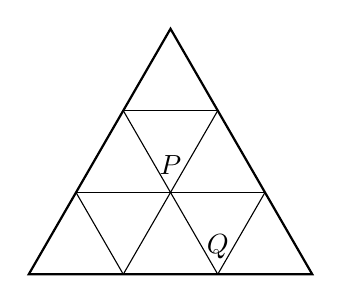
\begin{tikzpicture}[scale=1.2]
    \def\h{0.8660254}

    \draw[thick] (0,0) -- (3,0) -- (1.5, 3*\h) -- cycle;

    \draw (0.5, \h) -- (2.5, \h);
    \draw (1.0, 2*\h) -- (2.0, 2*\h);

    \draw (1,0) -- (2, 2*\h);
    \draw (2,0) -- (2.5, \h);

    \draw (2,0) -- (1, 2*\h);
    \draw (1,0) -- (0.5, \h);

    \node at (1.5, 1.333*\h) {$P$};
    \node at (2.0, 0.333*\h) {$Q$};
  \end{tikzpicture}
\end{figure}

\end{document}
